% $Id: INF_Poster_example.tex 7714 2011-08-31 17:34:46Z tkren $
%
% TU Wien - Faculty of Informatics
% poster template
%
% This template is using the beamer document class and beamerposter package, see
% <http://www.ctan.org/tex-archive/macros/latex/contrib/beamer/>
% <http://www.ctan.org/tex-archive/macros/latex/contrib/beamerposter/>
% <http://www-i6.informatik.rwth-aachen.de/~dreuw/latexbeamerposter.php>
%
% For questions and comments send an email to
% Thomas Krennwallner <tkren@kr.tuwien.ac.at>
%

\documentclass[final,hyperref={pdfpagelabels=true}]{beamer}

\usepackage{TUINFPST}

\usepackage{lipsum}
 
%\title[Computational Intelligence]{Interactive Computer Generated Architecture}
% if you have a long title looking squeezed on the poster, just force
% some distance:
\title[Software Engineering and Internet Computing]{%
    PURGE - Design and Implementation \\[0.2\baselineskip]%
    of a High-Level Graphics Engine% \\[0.2\baselineskip]%
}
\author[c.atesman@gmx.net]{Necdet Can Atesman}
\institute[]{%
  Technische Universit{\"a}t Wien\\[0.25\baselineskip]
  Institut f{\"u}r Computersprachen\\[0.25\baselineskip]
  Arbeitsbereich: Programmiersprachen und Übersetzer\\[0.25\baselineskip]
  Betreuer: a.o.Univ.Prof. DI Dr.tech. Franz Puntigam
}
\titlegraphic{
\includegraphics[height=52mm]{complang.eps}}
\date[\today]{\today}
\subject{epilog}
\keywords{my kwd1, my kwd2}

%%%%%%%%%%%%%%%%%%%%%%%%%%%%%%%%%%%%%%%%%%%%%%%%%%%%%%%%%%%%%%%%%%%%%%%%%%%%%%%%%%%%%%

% Display a grid to help align images 
%\beamertemplategridbackground[12.7mm]

% play around with the background colors
% \setbeamercolor{background canvas}{bg=yellow}

% use a background picture
% \usebackgroundtemplate{%
%   
\includegraphics[width=\paperwidth]{logo_KBS_2_CMYK}
% }

% play around with block colors
\setbeamercolor{block body}{fg=black,bg=white}
\setbeamercolor{block title}{fg=green,bg=white}

\setbeamertemplate{block begin}{
  \begin{beamercolorbox}{block title}%
    \begin{tikzpicture}%
      \node[draw,rectangle,line width=3pt,rounded corners=0pt,inner sep=0pt]{%
        \begin{minipage}[c][2cm]{\linewidth}
          \centering\textbf{\insertblocktitle}
        \end{minipage}
      };
    \end{tikzpicture}%
  \end{beamercolorbox}
  \vspace*{1cm}
  \begin{beamercolorbox}{block body}%
}

\setbeamertemplate{block end}{
  \end{beamercolorbox}
  \vspace{2cm}
}

% setup postit
\setbeamercolor{postit}{fg=black,bg=yellow} 
\newenvironment{postit}
{\begin{beamercolorbox}[sep=1em,wd=7cm]{postit}}
{\end{beamercolorbox}}

\definecolor{fade1}{rgb}{0.25,0.25,0.25}
\definecolor{fade2}{rgb}{0.5, 0.5, 0.5}
\definecolor{fade3}{rgb}{0.75,0.75,0.75}


% for crop marks, uncomment the following line
\usepackage[cross,width=88truecm,height=123truecm,center]{crop}

%%%%%%%%%%%%%%%%%%%%%%%%%%%%%%%%%%%%%%%%%%%%%%%%%%%%%%%%%%%%%%%%%%%%%%%%%%%%%%%%%%%%%%

\usepackage{listings}
	\lstloadlanguages{C++}
	\lstset{language=C++,basicstyle=\ttfamily\small}
	\lstnewenvironment{code}[1][]{\lstset{frame=rb,gobble=#1,tabsize=1,escapechar=!}}{}
	\lstnewenvironment{codeNoBorder}[1][]{\lstset{frame=,gobble=#1,tabsize=1,escapechar=!}}{}
	\lstset{tabsize=1,aboveskip=1.2em,belowskip=0.8em}

\newenvironment{smalllist}{\begin{list}{$\bullet$}{\itemsep 0cm \parskip 0pt}}{\end{list}}

\begin{document}

% We have a single poster frame.
\begin{frame}[fragile]

	\begin{columns}[t]
		\begin{column}{.3\textwidth}
			\begin{figure}[htbp]
				\centering
				
\includegraphics[width=246.3mm]{images/ogre/screenshot.jpg}
				\caption{Official Ogre3D tutorial}
			\end{figure}
		\end{column}
		\begin{column}{.65\textwidth}
			\begin{codeNoBorder}[0]
				Ogre::Root* root = new Ogre::Root();
				root->restoreConfig();
				root->initialise(false);
				auto window = root->createRenderWindow("Ogre RenderWindow", 800, 600, false);
				auto sceneMgr = root->createSceneManager(Ogre::ST_GENERIC);
				auto cam1 = sceneMgr->createCamera("cam1");
				auto camNode1 = sceneMgr->getRootSceneNode()->createChildSceneNode("camnode1");
				cam1->setNearClipDistance(5);
				!{\color{fade1}camNode1->attachObject(cam1);}!
				!{\color{fade2}camNode1->setPosition(100, 100, 100);}!
				!{\color{fade3}camNode1->lookAt(Ogre::Vector3(-1, -1, -1), Ogre::Node::TS\_LOCAL);}!
			\end{codeNoBorder}
		\end{column}
		%\begin{column}{.3\textwidth}
		%	\begin{figure}[htbp]
		%		\centering
		%		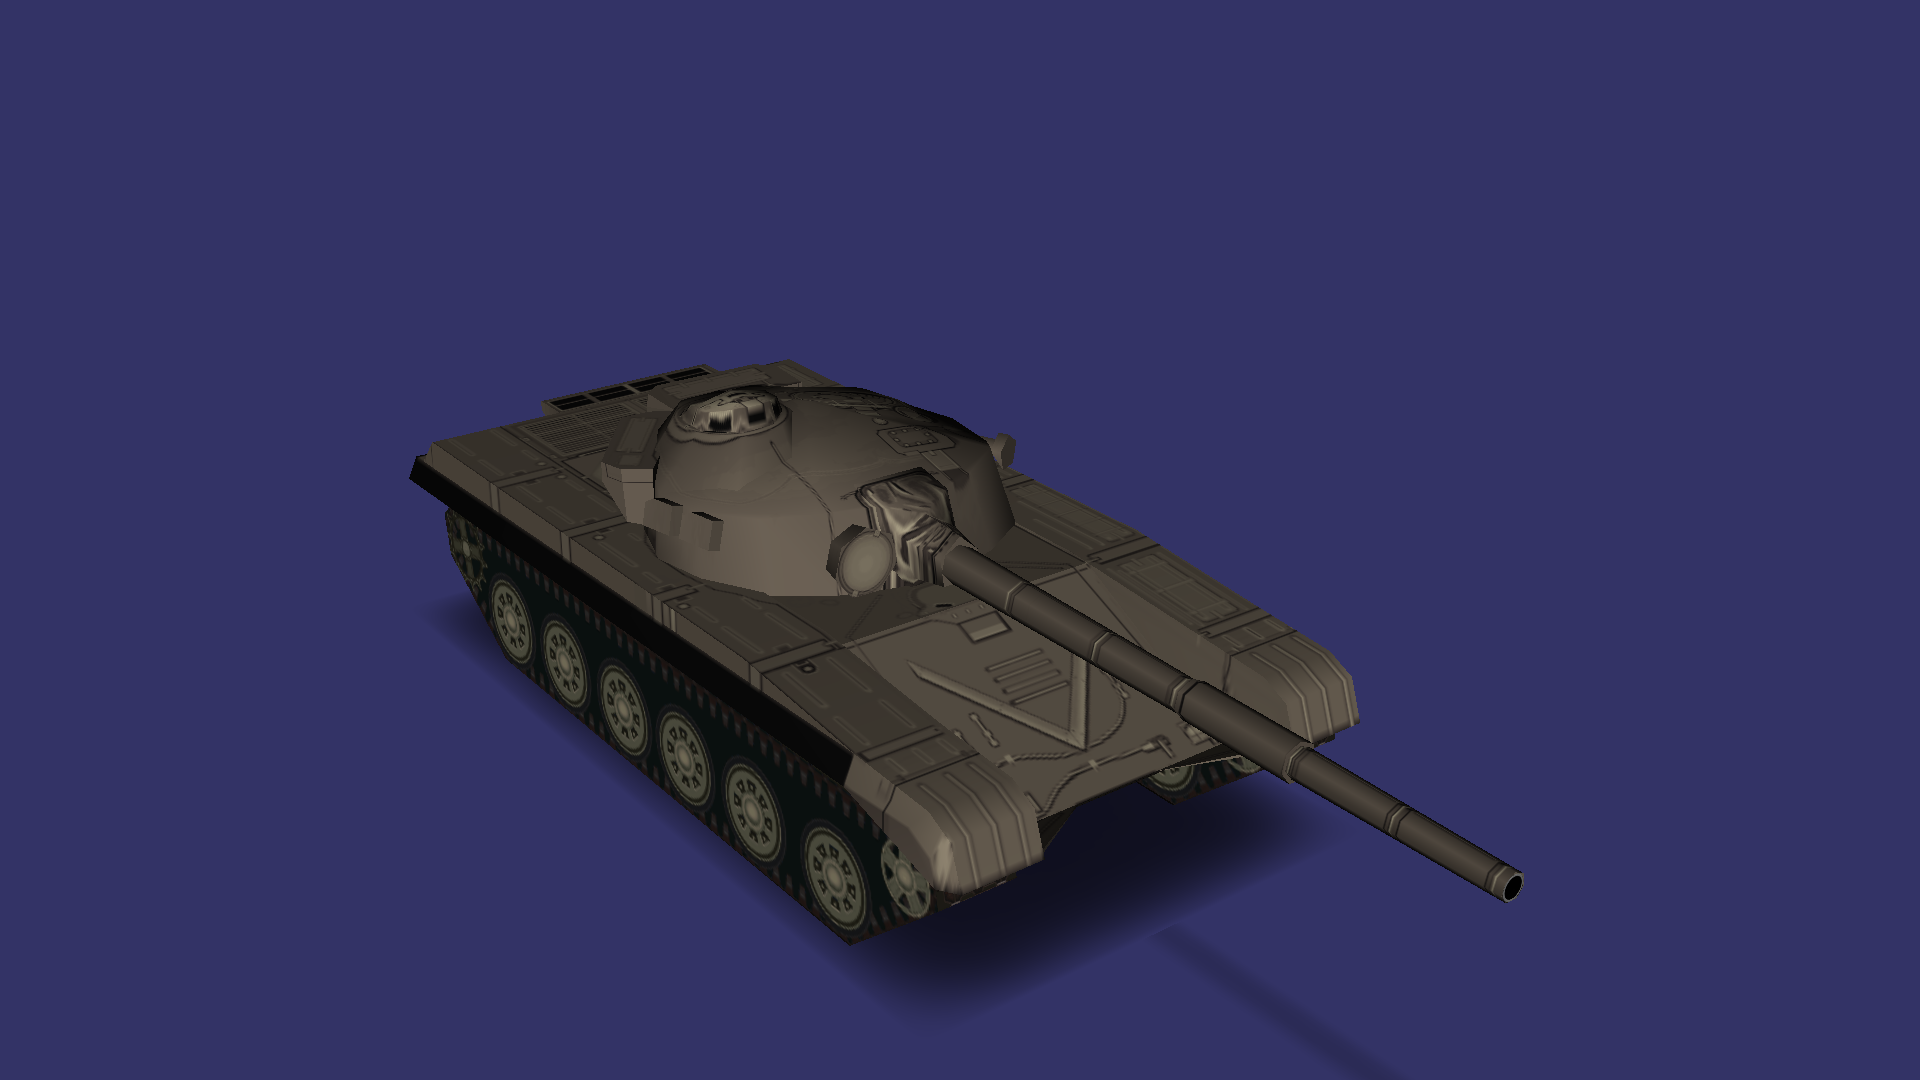
\includegraphics[width=246.3mm]{images/osg/screenshot.png}
		%		\caption{Official OpenSceneGraph tutorial}
		%	\end{figure}
		%\end{column}
		%\begin{column}{.3\textwidth}
		%	\begin{figure}[htbp]
		%		\centering
		%		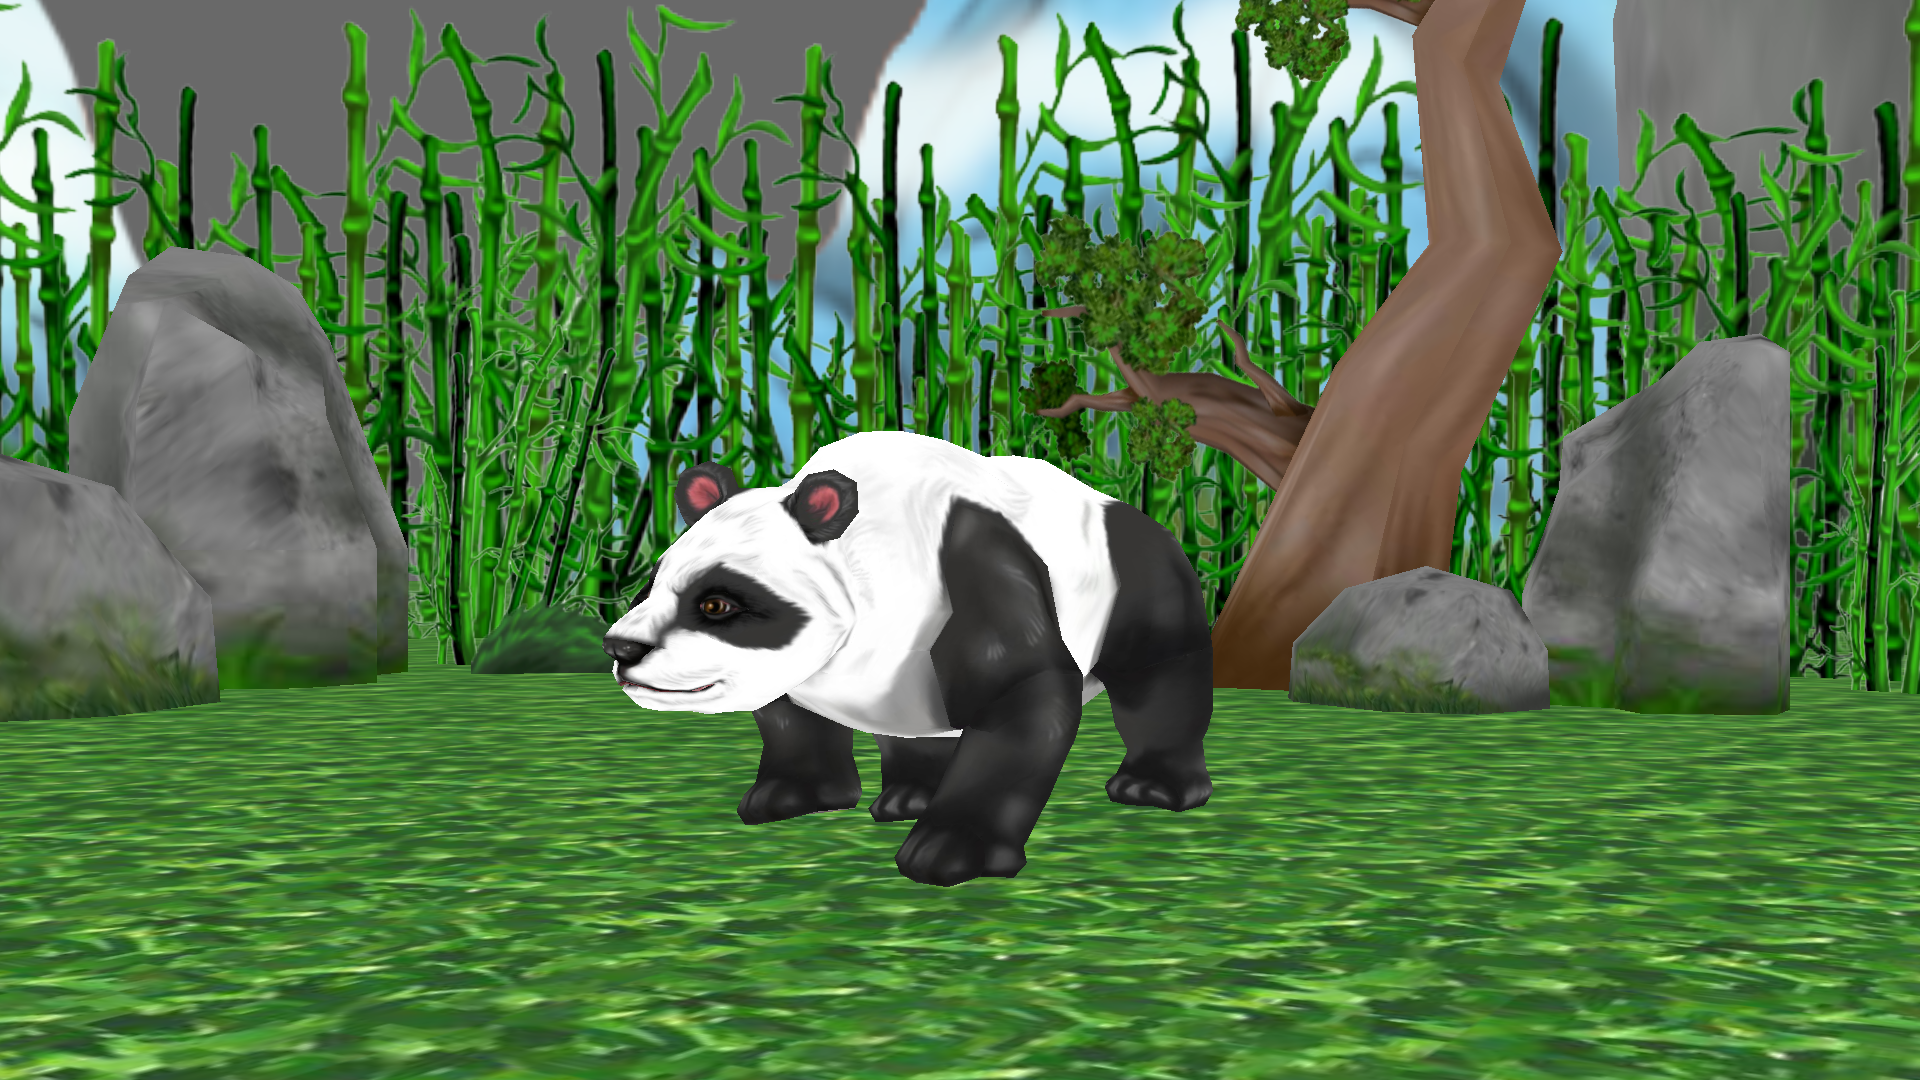
\includegraphics[width=246.3mm]{images/panda/screenshot.png}
		%		\caption{Official Panda3D tutorial}
		%	\end{figure}
		%\end{column}
	\end{columns}
	\begin{columns}[t]
		% ---------------------------------------------------------%
		% Set up a column
		\begin{column}{.45\textwidth}

			\begin{block}{Introduction}
				Our aim was to reduce the complexity present in modern graphics engine APIs for simple operations.
				\begin{smalllist}
					\item We have created s new API aimed at developers with no prior experience in graphics development for this purpose.
					\item We did not remove any concepts familiar to experienced developers, allowing optimizations at a later point.
				\end{smalllist}

			\end{block}

			\begin{block}{Innovations}
				The API exchanges readability and ease of use for performance:
				\begin{smalllist}
					\item Attitude in 3D-space is replaced by orientation in relative terms -- like turning left -- within a sub-space.
					\item Scene graph management is automated -- the focus during object management is kept on grouping and nesting instead.
					\item Sane defaults are implemented at various places. A render window will be created automatically if it was not created explicitly, for example.
					\item Support for discrete modification of objects through time -- like changing the color of a light within a given time frame.
					\item Fluent interfaces throughout the API.
				\end{smalllist}
			\end{block}

			\begin{block}{Performance}
				To be able to measure the performance impact of our API, we chose to use Ogre3D as the rendering engine. This enabled us to compare our performance measurements to an equivalent implementation in Ogre3D. We have found no significant performance loss in simple scenes, but the performance degraded as
				\begin{smalllist}
					\item the models became less complex, causing the renderer to spend more time processing updates to the objects in the scene than rendering them,
					\item and the scene became much more dynamic, when it consisted of hundreds of objects constantly changing their orientation.
				\end{smalllist}
				The results are very satisfactory nonetheless, as the aim was to provide an API for the simplest operations.
			\end{block}

		\end{column}
		% ---------------------------------------------------------%
		% end the column

		% ---------------------------------------------------------%
		% Set up a column 
		\begin{column}{.45\textwidth}

			\begin{block}{Code Sample}

				The following code is sufficient to load a model from a file, position the camera and render the scene from the viewpoint of the camera -- the output is seen in the lower right:

				\begin{code}[0]
					PURGEBridge::Ogre_1_7::OgreRenderer::createInstance();
					PURGE::Window::create(1920, 1080);
					PURGE::Camera::create()
					    ->move(100, 100, 100)
					    ->setDirection(-1, -1, -1);
					PURGE::Model::load("alexandria");
					PURGE::MainTaskGroup::get()->loop();
				\end{code}

				This is two to four times shorter than the minimal implementations using Ogre3D, Openscenegraph or Panda3D.

			\end{block}

			\begin{block}{Future Work}
				\begin{smalllist}
					\item This simplified API covers very few aspects of graphics engines. The addition of further features could create an engine that teaches the developer about advanced topics while he/she is using it.
					\item The current implementation using an external renderer adds an additional layer of complexity on top of Ogre3D. Optimizating the communication between these two software layers would lead to much higher performance rates.
					\item Another interesting feature that emerged during the implementation is the ability to exchange the underlying graphics engine at runtime. It would be possible to provide a unified API to multiple graphics engines using this architecture.
				\end{smalllist}
			\end{block}

			%\begin{block}{References}
			%	% this is just an example, use BibTeX!
			%	\begin{thebibliography}{999}
			%		\bibitem[Foo~and~Fu, 2010]{ff2010}
			%			Foo, B.; and Fu, B.
			%			2010.
			%			\newblock {On logical representations of hackerisms}.
			%			{\em J.~Log.~Hack.} 1:1--2.
			%		\bibitem[Crock~et~al., 2010]{ck2010}
			%			Crock, A; Cruft, B.; and Kludge, C.
			%			2010.
			%			\newblock {Decomposing junk code}.
			%			Manuscript.
			%	\end{thebibliography}
			%\end{block}

			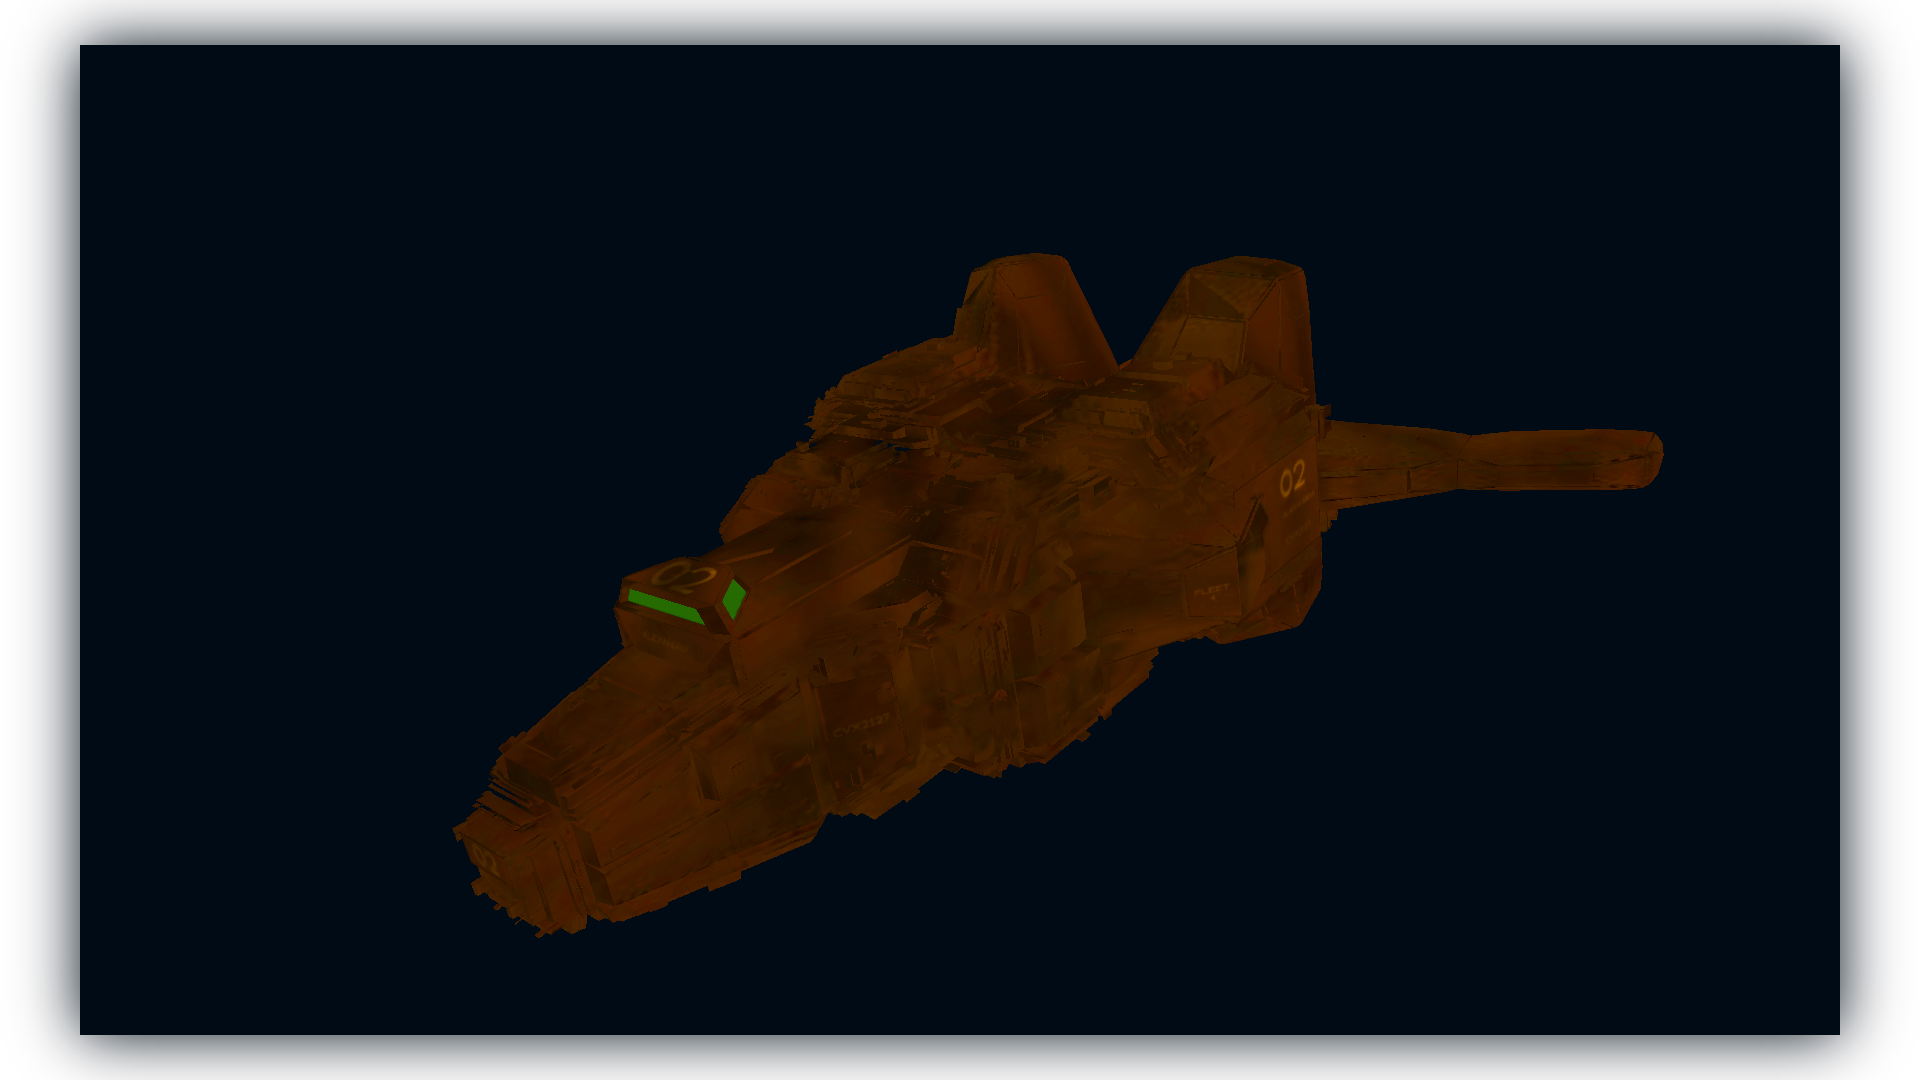
\includegraphics[width=369.5mm]{images/PURGE.png}

		\end{column}
		% ---------------------------------------------------------%
		% end the column
	\end{columns}

  %\begin{tikzpicture}[remember picture,overlay]
  %  \node[inner sep=0pt,xshift=-30cm,yshift=23cm] at (current page.east) {%
  %    \begin{postit}%
  %      Post-It time!%
  %    \end{postit}%
  %  }; 
  %\end{tikzpicture}
  
\end{frame}

\end{document}

%%% Local Variables:
%%% TeX-PDF-mode: t
%%% TeX-debug-bad-boxes: t
%%% TeX-master: t
%%% TeX-parse-self: t
%%% TeX-auto-save: t
%%% reftex-plug-into-AUCTeX: t
%%% End:
